\chapter{Project Plan}
This section is an excerpt of the project plan. The project plan features descriptions of which experiments, technologies etc. to conduct, investigate and implement during the Bachelor's Project. \newline

This section contains how the project work will be structured, which methods to be used, etc. \newline

\subsection{The Bachelor's Project}
The Bachelor’s Project (Thesis or Final Project) is an extensive project dealing with a realistic engineering assignment. The bachelor project should document the students’ ability to work independently to apply engineering methods and theories in solving professional problems and development issues in a specific field. The project constitutes the conclusion of the programme and is placed in the last semester. \newline

The Bachelor's Project workload is \textbf{20 ECTS points}. \textbf{1 ECTS} translates to \textbf{27 hours of workload}, totaling \textbf{540 hours} of workload for the Bachelor's Project. Assuming 18 weeks of Bachelor's Project work, total workload/week is ~30 hours/week. \newline

During the project period, 2 elective courses with 10 ECTS points in total to fulfill the goal of 30 ECTS workload each semester. Assuming 18 weeks of lectures and homework assignments and projects, total workload/week is ~16-17 hours/week. \newline

Total workload is therefore expected to be ~45-50 hours/week during the semester. To keep track of the project, weekly SCRUM meetings with supervisor is essential along with project management tools: \\

- The ASE-model \\
- SCRUM \\
- Redmine \newline

\subsection{ASE-model}

\begin{figure}[H]
\centering
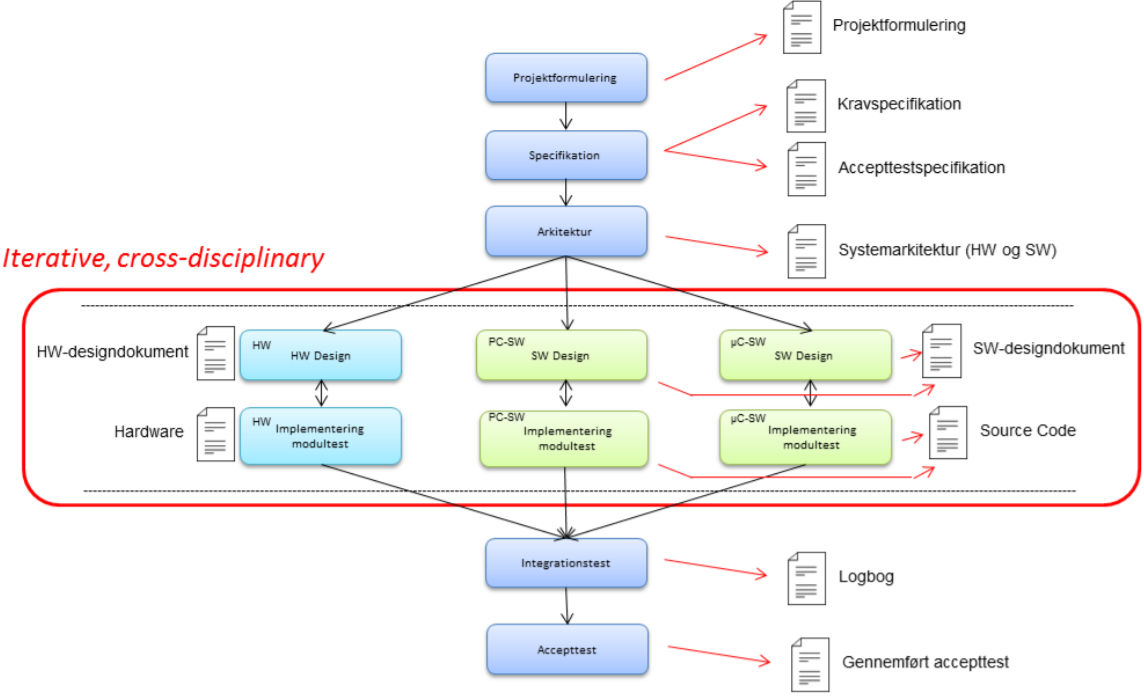
\includegraphics[scale=0.4]{./pictures/ASEmodel.png}
\caption{The Aarhus School of Engineering model - The ASE-model.}
\label{fig:ASEmodel.png}
\end{figure}

The figure above is the ASE-model that engineering students at Aarhus School of Engineering (ASE) was introduced to during their 2nd semester. The ASE-model is a structured model for design and development of hardware- and software-systems. \newline

A project of this magnitude contain and introduce several new technologies, with it many technical and project risks during the project work. Thus, an iterative project procedure is a helpful tool to ensure a clear procedure, as the beginning a new projects is usually difficult, necessitates management and overview to prevent wasting time on unnecessary activities. \newline

The iterative, cross-disciplary model is useful when designing domain, technology, implementation possibilities, etc. Designing a system using the ASE-model reduces possible project risks and enables the option to specify requirements, formulate tests and design complete use-cases early in the project. Combining the ASE-model with an iterative process, the project process is robust from project risks and future modfications. \newline

An iterative process produces functional product parts by completing tasks \textit{piece by piece} (iterations) for each module of the project. Using this method, an early assessment of project success is possible along with an early risk prevention assessment. \newline

Every iteration contains elements from several processes outlined in the ASE-model. Hence, an iteration can contain both design, implementation and test for a minor part of the project. \\

\subsubsection{Iterative development with the ASE-model}
Even though a team chooses an iterative process, the project still has various phases as shown in Figure ~\ref{fig:ASEmodel.png}. The first iterations' focus is primarily a description of idea and establishing project requirements. The following iterations focuses on system development before moving on to implementation. \\
The difference between an iterative process and the ASE-model in Figure ~\ref{fig:ASEmodel.png} is that we operate in \textit{parallel} on several types of tasks within a given iteration. This is ongoing to better build, modify and refine the product on the basis of experiences and discoveries from earlier iterations. \newline

For instance, the initial iterations outlines the first and the most important project requirements. When the reuirements are established, the problem domain is investigated: 'How can we implement GUI on a PC laptop?', 'How to measure Total Harmonic Distortion (THD) on audio output?, 'How do we establish USB-connection between GUI and Showman?', etc. \\
This iteration helps clarifying the thesis statement and allows the team the opportunities to conduct physical tests. \newline

In each iteration, the team works on almost every project area. Documentation is produced during the process and needs to be regularly updated. \\ 

\subsection{SCRUM}
SCRUM is used to manage the iterative process. The reason is the welldocumented work procedures and team roles. Organizing the project by using SCRUM gives the project a clear overview and keeps the work flow going, even though external activities such as other courses can distract the process - In short, SCRUM makes the project manageable as the teams works toward small, but clear goals. Another reason is the widely accepted use of SCRUM in companies, giving the team necessary introduction and experience in using SCRUM. \newline

The project team defines a framework with a set of \textbf{milestones} with mandatory assignments for each milestone, but gives the team the freedom to reach these milestones. \newline

Even though SCRUM is an integral part of project work at ASE, a detailed analysis and discussion of SCRUM is not within the scope of this document. The following is brief overview of selected elements of SCRUM. \newline

\subsubsection{Milestones}
The table in Figure ~\ref{fig:milestonespng}below outlines the typical milestones for a project at ASE, weeknumbers relative to semesterstart:

\begin{figure}[H]
\centering
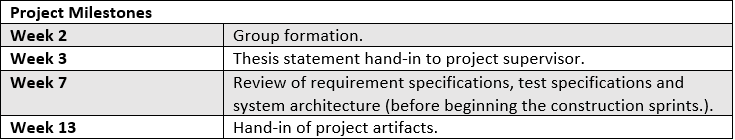
\includegraphics[scale=0.8]{./pictures/milestones.png}
\caption{Example of SCRUM milestones.}
\label{fig:milestonespng}
\end{figure}

\subsection{Redmine}


\subsection{Supervisor Meetings}


\subsection{Timetable}


%\textbf{Objective} \\
%The objective of the Bachelor’s Project is that students be able to plan and conduct an engineering project in as realistic a form as the study environment allows, preferably in cooperation with companies. \\

%\textbf{Learning Objectives} \\
%Upon completion of the Bachelor’s Project, the student should be able to: \\

%- Apply scientific research results and technological knowledge for solving  technical problems, \\
%- Develop new solutions, \\
%- Acquire and evaluate new knowledge within relevant engineering fields, \\
%- Systematically apply engineering knowledge, theories and methods \\
%- Plan and complete a project in a group in cooperation with internal and external partners \\
%- Present results of a project in writing and orally by means of relevant communication tools, to professionals as well as customers, \\
%- Present results of a project orally and with means of various audio or visual communication tools, \\
%- Integrate social, economic, environmental and work environmental consequences in the solution model \newline

%Learning objectives in relation to the specific subject and with reference to above, including their weight, is specified in the Assignment Formulation. \newline

%\textbf{Main Content} \\
%The Bachelor’s Project should comprise the planning and documentation of solutions for a realistic engineering project or defined parts and comprise independent experimental, empirical and/or theoretical discussions and computations. \\

%\subsection{Project Plan}
%Project management tools are needed for the project to keep focus. Aarhus School of Engineering development model 